\section{Concurrent Prime Sieve (primes.c)}

\subsection{Ý tưởng thiết kế và Mô hình hoạt động}
Chương trình hiện thực thuật toán Sàng Eratosthenes đồng thời (\textit{Concurrent Prime Sieve}) dựa trên mô hình xử lý luồng dữ liệu qua chuỗi đường ống dẫn (\textit{concurrent pipeline}). 

Ý tưởng kết hợp đường ống Unix (\textit{pipe}) với thuật toán sàng số nguyên tố xuất phát từ đề xuất mang tính nền tảng của Doug McIlroy --- nhà khoa học máy tính tại Bell Labs và là người phát minh ra khái niệm Unix Pipeline \cite{mcilroy1968coroutines, mcilroy1978unix}. Mô hình này đại diện cho kiến trúc tính toán dòng dữ liệu CSP (\textit{Communicating Sequential Processes}) được khởi xướng bởi C. A. R. Hoare \cite{hoare1978csp}, đồng thời vận dụng trực tiếp các cơ chế quản lý tiến trình và giao tiếp liên tiến trình (IPC) trong hệ điều hành xv6 \cite{xv6book, remzi2018ostep}.

\begin{figure}[H]
    \centering
    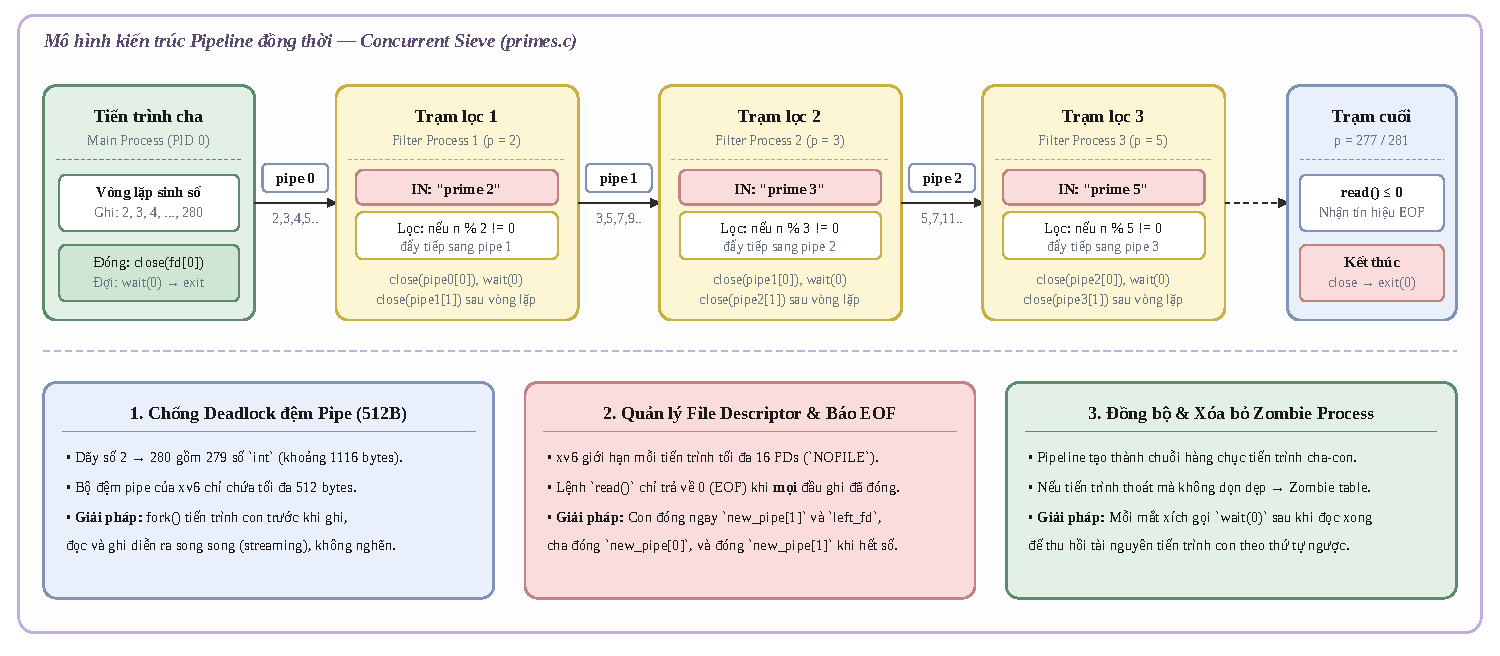
\includegraphics[width=\textwidth]{images/primes_pipeline.pdf}
    \caption{Mô hình luồng dữ liệu đường ống và các giải pháp hệ thống trong \texttt{primes.c}}
    \label{fig:primes_pipeline}
\end{figure}

\noindent Luồng thực thi diễn ra tuần tự qua các giai đoạn:
\begin{itemize}
    \item \textbf{Tiến trình khởi tạo (Main Process):} Tạo \code{pipe 0}, thực hiện \code{fork()} để tạo tiến trình con lọc đầu tiên, sau đó ghi dãy số từ $2$ đến $280$ vào đầu ghi của \code{pipe 0}.
    \item \textbf{Các trạm lọc trung gian (Filter Stages):} Mỗi tiến trình đọc số nguyên đầu tiên $p$ từ pipe bên trái (\code{left\_fd}). Số $p$ này chắc chắn là số nguyên tố và được in ra màn hình. Kế tiếp, tiến trình tạo một pipe mới (\code{new\_pipe}), \code{fork()} tiến trình con kế tiếp, rồi đóng vai trò lọc: đọc các số $n$ còn lại, nếu $n \pmod p \neq 0$ thì đẩy vào \code{new\_pipe}.
    \item \textbf{Trạm kết thúc (Termination):} Khi đường ống bên trái đóng hoàn toàn, hàm \code{read()} trả về giá trị $\le 0$ (EOF). Tiến trình thực hiện đóng đầu pipe, gọi \code{wait(0)} để đợi tiến trình con và thoát an toàn.
\end{itemize}

\subsection{Khó khăn kỹ thuật và Giải pháp thực tế}
Dựa trên các đặc thù kiến trúc và giới hạn tài nguyên của hệ điều hành xv6 \cite{xv6book}, bài làm đã giải quyết ba thách thức then chốt:
\begin{enumerate}
    \item \textbf{Ngăn ngừa Deadlock do bộ đệm Pipe giới hạn (512 bytes):} 
    Dãy số $2 \to 280$ tương ứng hơn $1.1\text{ KB}$ dữ liệu, vượt quá dung lượng đệm của một pipe trong xv6. Nếu tiến trình cha ghi toàn bộ dữ liệu trước khi con đọc, lời gọi \code{write()} sẽ bị chặn vô tận (\textit{blocked}) gây treo hệ thống. \\
    \textit{Giải pháp:} Khởi tạo \code{fork()} trước khi bắt đầu ghi, giúp luồng dữ liệu được tiêu thụ đồng thời dạng streaming.
    \item \textbf{Quản lý File Descriptor và tín hiệu ngắt EOF:}
    Hàm \code{read()} chỉ trả về 0 khi toàn bộ các đầu ghi của pipe đó được đóng. Nếu tiến trình con không đóng đầu ghi thừa kế thừa từ cha, lệnh \code{read()} sẽ chờ vĩnh viễn. Ngoài ra, xv6 giới hạn mỗi process chỉ có 16 FDs (\code{NOFILE}). \\
    \textit{Giải pháp:} Tiến trình con lập tức \code{close(new\_pipe[1])} và \code{close(left\_fd)}; tiến trình cha \code{close(new\_pipe[0])} và \code{close(new\_pipe[1])} ngay sau khi đẩy hết dãy số.
    \item \textbf{Thu dọn tài nguyên tiến trình con (Zombie Process):}
    Tất cả các tiến trình cha trong chuỗi đều gọi lệnh \code{wait(0)} trước khi kết thúc, đảm bảo bảng tiến trình của hệ điều hành được dọn dẹp sạch sẽ theo khuyến nghị quản lý tiến trình \cite{remzi2018ostep}.
\end{enumerate}

\newpage

\section{Directory Tree Visualization (tree.c)}

\subsection{Ý tưởng thiết kế và Cơ chế Lookahead Buffer}
Lệnh \code{tree} mô phỏng tiện ích dòng lệnh kinh điển trên hệ thống Unix/Linux do Steve Baker phát triển \cite{baker1996tree}. Chương trình duyệt hệ thống tệp đệ quy theo chiều sâu (DFS), hỗ trợ hiển thị cấu trúc phân nhánh đẹp mắt cùng các cờ tùy chọn \code{-L <depth>} (giới hạn độ sâu) và \code{-d} (chỉ hiển thị thư mục). Cấu trúc \texttt{struct dirent} và bảng chỉ mục \texttt{inum} được truy xuất trực tiếp từ hệ thống tệp tin xv6 \cite{xv6book}.

\begin{figure}[H]
    \centering
    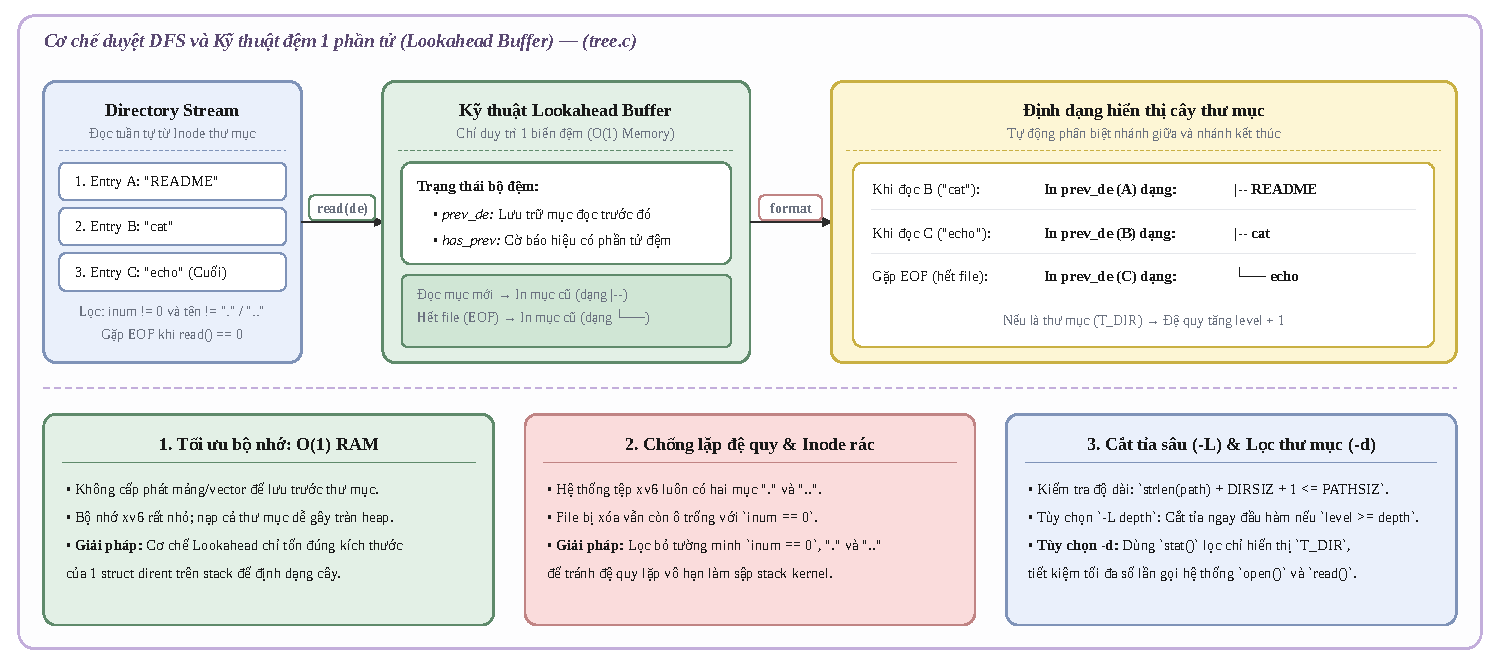
\includegraphics[width=\textwidth]{images/tree_lookahead.pdf}
    \caption{Cơ chế Lookahead Buffer $O(1)$ RAM và định dạng cây thư mục trong \texttt{tree.c}}
    \label{fig:tree_lookahead}
\end{figure}

\subsection{Điểm sáng giải thuật và Xử lý ca biên}
\begin{enumerate}
    \item \textbf{Kỹ thuật đệm 1 phần tử (1-Item Lookahead Buffer) đạt $O(1)$ bộ nhớ:}
    Để vẽ đúng định dạng cây chuẩn Unix (phần tử giữa dùng \texttt{|--}, phần tử cuối dùng \texttt{\textbackslash{}\_\_\_}), phương pháp thông thường cần nạp toàn bộ danh sách tệp vào mảng/vector để biết chỉ số cuối cùng. Trong môi trường nhúng có bộ nhớ hạn hẹp như xv6, giải pháp này dễ dẫn đến tràn bộ nhớ heap. \\
    \textit{Giải pháp:} Sử dụng bộ đệm chỉ gồm 1 phần tử (\code{prev\_de}, \code{prev\_stat}). Khi đọc một entry hợp lệ mới từ thư mục, chương trình mới in entry trước đó bằng ký hiệu \texttt{|--}. Khi gặp EOF (hết thư mục), entry đang nằm trong bộ đệm chắc chắn là phần tử cuối cùng và được in bằng \texttt{\textbackslash{}\_\_\_}.
    \item \textbf{Chống lặp đệ quy vô hạn và loại bỏ Inode rác:}
    Hệ thống tệp Unix luôn chứa hai liên kết đặc biệt là \texttt{"."} và \texttt{".."}. Chương trình chủ động lọc bỏ hai mục này và các ô inode trống (\code{inum == 0}) để bảo vệ stack kernel không bị tràn.
    \item \textbf{Kiểm soát độ dài đường dẫn và cắt tỉa đệ quy:}
    \begin{itemize}
        \item Kiểm tra an toàn trước khi ghép chuỗi: \code{strlen(path) + DIRSIZ + 1 <= PATHSIZ}.
        \item Tùy chọn \code{-L depth}: Dừng đệ quy sớm ngay từ điều kiện dừng (\textit{base case}) \code{level >= max\_depth}, tránh việc thực hiện lời gọi hệ thống \code{open()} không cần thiết.
        \item Tùy chọn \code{-d}: Dùng \code{stat()} kiểm tra kiểu inode (\code{T\_DIR}), lọc bỏ tệp tin ngay trong vòng lặp đọc.
    \end{itemize}
\end{enumerate}

\subsection{Kết quả thực nghiệm}
Chương trình hoàn thành xuất sắc các ca kiểm thử: chạy mặc định \code{tree}, giới hạn độ sâu \code{tree -L 2}, lọc thư mục \code{tree -d}, và chỉ định đường dẫn cụ thể mà không gặp bất kỳ lỗi rò rỉ bộ nhớ hay cạn kiệt file descriptor.
